\section{Calibration of electromagnetic objects}
\frame{\tableofcontents[currentsection]}
%%=============================
\begin{frame}{Full calibration}
  To reach the physics analyses, data and simulated reconstructed events must pass a calibration procedure.
  This procedure aims at correcting the measured energy to \textcolor{blue}{\bf retrieve the true energy of the particle at the interaction point}.
  \begin{center}
    \begin{tikzpicture}
      \node[anchor=south west] {\includegraphics[width=\linewidth]{ATL-COM-PHYS-2013-1653_1f.pdf}};
%%      \draw[step=1.0,black,thin] (0,0) grid (30,10);
%%      \draw[red, line width=1mm, rounded corners =2pt] ( 20.5, 2.6 ) rectangle ( 24.3, 11 ) ;
      \end{tikzpicture}
  \end{center}
  Electrons and photons follow the same steps but with dedicated analyses. 
%%This analysis continues work from JB Blanchard \& JB de Vivie : \href{https://cds.cern.ch/record/1637533/files/ATL-COM-PHYS-2013-1653.pdf}{\bf ATL-COM-PHYS-2013-1653}.
\end{frame}
%%=============================
%========================
\begin{frame}{MVA calibration}
\begin{itemize}
\item Simulated events are passed through a full GEANT4 simulation of the ATLAS detector.
\item Events are then categorized in $\eta$ and $p_T$ bins, separately for electrons and photons.
\item \textcolor{blue}{\bf A multivariate analysis (MVA), using ECAL variables, is performed to compute the true energy from detector observables}.
\end{itemize}

  %% \begin{minipage}{0.49\linewidth}
  %%   MVA uses :
  %%   \begin{itemize}
  %%   \item Energies in all layers of the ECAL
  %%   \item EM shower shape variables
  %%   \item Barycenters of energy deposits
  %%   \end{itemize}
  %% \end{minipage}
  %% \hfill
  %% \begin{minipage}{0.49\linewidth}
\begin{center}
  Most probable value (MPV) of $E^{corr}/E^{true}$.\\
  \includegraphics[width=0.5\linewidth]{CERN-PH-EP-2014-153_2fa.pdf}
\end{center}
%  \end{minipage}

\end{frame}
%=================================
\begin{frame}{Energy scale factors}
  \begin{minipage}{0.49\linewidth}
    After MVA calibration, mass distribution of $Z\rightarrow ee$ for data and MC still have {\bf discrepancy}.
    \newline
    \textcolor{blue}{\bf A data-driven analysis } is performed to match data to MC distribution (relative matching).
  \end{minipage}
  \hfill
  \begin{minipage}{0.49\linewidth}
    \includegraphics[width=\linewidth]{CalibSupNote_Distri_m12_uncorrected.pdf}
  \end{minipage}

A correction, applied to both electrons of Z decay, is computed to \textcolor{red}{\bf shift the central value of data distribution} : 
\begin{center} \textcolor{blue}{\bf energy scale factor ($\alpha$)} \end{center}
$$E^{corr}=E^{meas}(1+\alpha)$$
\end{frame}

%%============================
\begin{frame}{Resolution constant term}
  \input{/home/goudet/Documents/LAL/ExternalPlot/ResolutionConstantTerm.tex}
  \begin{itemize}
  \item $a$ : sampling term ( $10\%$). Linked to the fluctuations of electromagnetic showers. \\Can be simulated.
  \item $b$ : noise + pile-up term ( $\sim 350~cosh(\eta )$~MeV ). Measured in dedicated runs.
  \item $c'$ : simulated constant term
  \item {\bf $c$ : in-situ additional constant term ($0.7\%$)}
  \end{itemize}
  We observe that data distribution is larger than MC. 
  $c$ is measured to enlarge MC up to the data width.
  Both MC electrons undergo the correction :
  \begin{center}\textcolor{blue}{\bf Resolution constant term ($c$) }\end{center}
  $$E^{corr} = E^{meas}(1+N(0,1)*c)$$
  $N(0,1)$ : a Gaussian distributed random number
\end{frame}

%%===================================
\begin{frame}{Template method}
  The template method is used to measure $\alpha$ and $c$ simultaneously.
  \begin{itemize}
  \item Create distorded MC (templates) with test values of $\alpha$ and $c$
  \item \textcolor{blue}{\bf Compute $\chi^2( M_Z; \text{data, template})$}
  \item \textcolor{blue}{\bf Fit the minimum of the $\chi^2$ distribution} in the ($\alpha,c$) plane.
  \end{itemize}
  \hfill
  \includegraphics[width=0.49\linewidth]{MC6_0_0_CompareAlpha.pdf}
  \includegraphics[width=0.49\linewidth]{MC6_0_0_chiMatrix.pdf}
\end{frame}

%========================================
\begin{frame}{Detector splitting}
  \begin{minipage}{0.49\linewidth}
    \includegraphics[width=\linewidth]{ATLASCaloPerf_2fi.pdf}
  \end{minipage}
  \begin{minipage}{0.49\linewidth}
    \begin{itemize}
    \item Detector is not uniform along $\eta$.
    \item To improve resolution, \\ \textcolor{blue}{\bf calibration is performed in bins of $\eta_{calo}$.}
    \item 68 and \textcolor{brown}{24} bins are used respectively for $\alpha$ and $c$.\\
    \end{itemize}
  \end{minipage}
  \vfill
  {\bf Electrons are labelled by their $\eta$ bin}, hence Z are labeled by the combination $(i, j)$ of electrons bins.
  \textcolor{blue}{\bf Scales are computed for each combination.}
\end{frame}

%============================

\begin{frame}{Inversion Procedure}
Obtaining \textcolor{blue}{\bf electron scales ($\alpha_i$) from Z scales ($\alpha_{ij} \pm \Delta\alpha_{ij}$)} need the minimizations of the following $\chi^2$'s.\\
\begin{minipage}{0.49\linewidth}
  $$\alpha_{ij} = \frac{\alpha_i+\alpha_j}{2}$$
  $$\chi^2 = \sum \limits_{i, j\leq i} \frac{ (\alpha_i + \alpha_j - 2\alpha_{ij})^2 }{(\Delta\alpha_{ij})^2}$$
  \includegraphics[width=\linewidth]{Closure24_alpha.pdf}
\end{minipage}
\hfill
\begin{minipage}{0.49\linewidth}
  $$c_{ij}^2 = \frac{c^2_i + c_j^2}{2}$$
  $$\chi^2 = \sum \limits_{i, j\leq i} \frac{ (\sqrt{\frac{c_i^2 + c_j^2}{2}} - c_{ij})^2 }{\Delta^2 c_{ij}}$$
  \includegraphics[width=\linewidth]{Closure24_c.pdf}
\end{minipage}

\end{frame}

%%===================================
\begin{frame}{Run 2 pre-recommandations}
  Run 2 early analyses need scales factors for 13~TeV but not enough were available.
  Need to \textcolor{blue}{ \bf estimate Run 2 scales from run 1 data}.
  \newline
  Pre-recommandations are computed using $8$~TeV data reprocessed with :
  \begin{itemize}
  \item new detector geometry (IBL)
  \item new reconstruction algorithm (4 samples)
  \item new calibration machine learning
  \end{itemize} 
  \begin{minipage}{0.49\linewidth}
    \begin{tikzpicture}
      \node[anchor=south west] {\includegraphics[width=\linewidth]{/home/goudet/Documents/LAL/Shared/PlotsGoudet/Calibration/PreRecommandations/PreRec_Zee_alpha.pdf}};
%      \draw[step=1.0,black,thin] (0,0) grid (2,2);
      \node[draw] at (3,2.5) {$\alpha$};
    \end{tikzpicture}
  \end{minipage}
  \begin{minipage}{0.49\linewidth}
    \centering
    \begin{tikzpicture}
      \node[anchor=south west] {    \includegraphics[width=\linewidth]{/home/goudet/Documents/LAL/Shared/PlotsGoudet/Calibration/PreRecommandations/PreRec_c.pdf}};
      \node[draw] at (3,2.5) {$c$};
    \end{tikzpicture}
  \end{minipage}
  %Binning was changed from $34$ bins to $68$ due to the observation of sub-structures.
\end{frame}

%%========================================

\begin{frame}{Calibration in-situ : run 2 pre-recommandations systematics}
2012 systematics are used for the pre-recommandations. \\
{\bf Two more systematics are added in quadrature } :
\begin{itemize}
\item Increasing the number of bin for $\alpha$ shows sub-patterns. 
  Systematic is defined as difference between a bin value and the average of its sub-bins.
\item Pre-recommandations being computed with 8TeV datasets, one needs to evaluate the impact of the center of mass energy.
Systematic is defined as the scale measured from $13$~TeV MC on $8TeV$ templates.
\end{itemize}
  \begin{minipage}{0.49\linewidth}
    \includegraphics[width=\linewidth]{/home/goudet/Documents/LAL/Shared/PlotsGoudet/Calibration/PreRecommandations/PreRecSyst_alpha.pdf}
  \end{minipage}
  \hfill
  \begin{minipage}{0.49\linewidth}
    \includegraphics[width=\linewidth]{/home/goudet/Documents/LAL/Shared/PlotsGoudet/Calibration/PreRecommandations/PreRecSyst_c.pdf}
  \end{minipage}\\
\end{frame}

%%===================================
\begin{frame}{Run 2 results}
  \begin{itemize}
  \item $\alpha$ measured independently for each year.
  \item $c$ measured on combined data.
    \end{itemize}

  \begin{minipage}{0.49\linewidth} 
    \includegraphics[width=\linewidth]{CalibSupNote_CS_alphaOff.pdf}
  \end{minipage}
  \hfill
  \begin{minipage}{0.49\linewidth}
    \includegraphics[width=\linewidth]{CalibSupNote_CS_cOff.pdf}
  \end{minipage}

    \begin{center}
    \begin{minipage}{0.7\linewidth}
      \centering
      {\bf Main sources of uncertainty }
      \begin{itemize}
      \item Diff. btw tight and medium electrons
      \item Closure : difference between injected and measured values
      \item Bremsstrahlung impact on electron momentum
      \end{itemize}
    \end{minipage}
  \end{center}

\end{frame}
%===============================================
\begin{frame}{Closure uncertainty}
  \centering
  \begin{minipage}{0.9\linewidth}
    \begin{itemize}
    \item Run 1 closure systematic defined on single measurement
    \item Run 2 cross-checks favoured opposite sign effect
    \item \textcolor{blue}{\bf Dominant resolution systematic requires more care}
    \end{itemize}
  \end{minipage}
  \\
  \begin{minipage}{0.49\linewidth}
    \includegraphics[width=\linewidth]{ATL-COM-PHYS-2013-1653_6b.pdf}
  \end{minipage}
\end{frame}
%===============================================
\begin{frame}{Run 2 closure uncertainty}
  \begin{itemize}
  \item Pseudo experiments have been performed
  \item Average over all sources of statistical fluctuations
  \item {\bf New closure defined as average of distribution in each bin.}
  \end{itemize}
  \centering
  \includegraphics[width=0.7\linewidth]{statTree_9775706_iBin_2_SAME.pdf}
\end{frame}
%===============================================
\begin{frame}{Comparing closure uncertainties}
  \centering
  {\bf Closure uncertainty}\\
  \begin{minipage}{0.42\linewidth}
    \includegraphics[width=\linewidth]{Clos_syst_alpha.pdf}\\
  \end{minipage}
  \hfill
    \begin{minipage}{0.42\linewidth}
    \includegraphics[width=\linewidth]{Clos_syst_c.pdf}\\
  \end{minipage}
    \newline
    {\bf Total uncertainty}\\
    \begin{minipage}{0.42\linewidth}
      \includegraphics[width=\linewidth]{run1Syst_alpha.pdf}\\
    \end{minipage}
    \hfill
    \begin{minipage}{0.42\linewidth}
      \includegraphics[width=\linewidth]{run1Syst_c.pdf}\\
    \end{minipage}

\end{frame}
%===============================================
\begin{frame}{Runs comparison}
  Performances of run 2 in-situ calibration better than Run 1.
  Cross-checks performed on photons from $Z\rightarrow ll\gamma$.\\
  \begin{minipage}{0.42\linewidth} 
    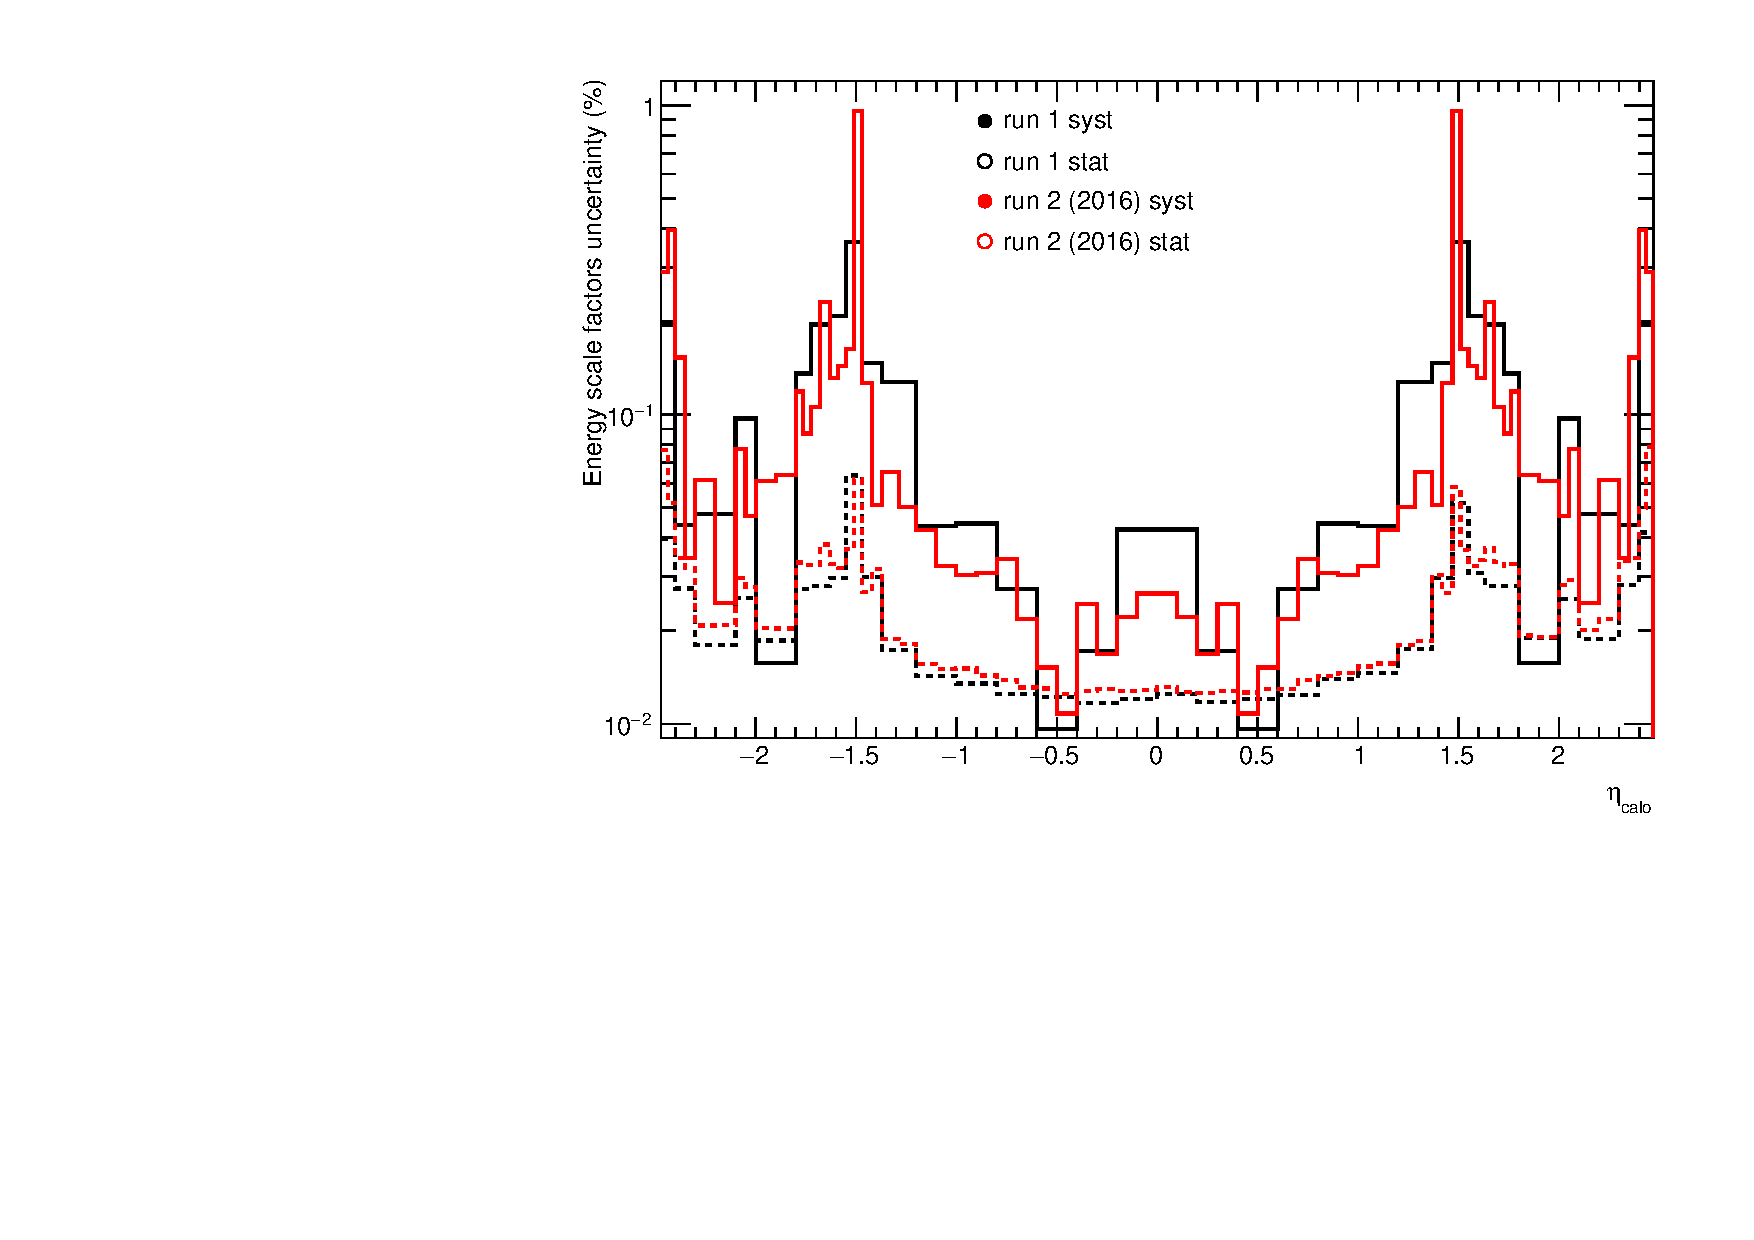
\includegraphics[width=\linewidth]{Figures/CompareSystRun_alpha.pdf}
  \end{minipage}
  \hfill
  \begin{minipage}{0.42\linewidth}
    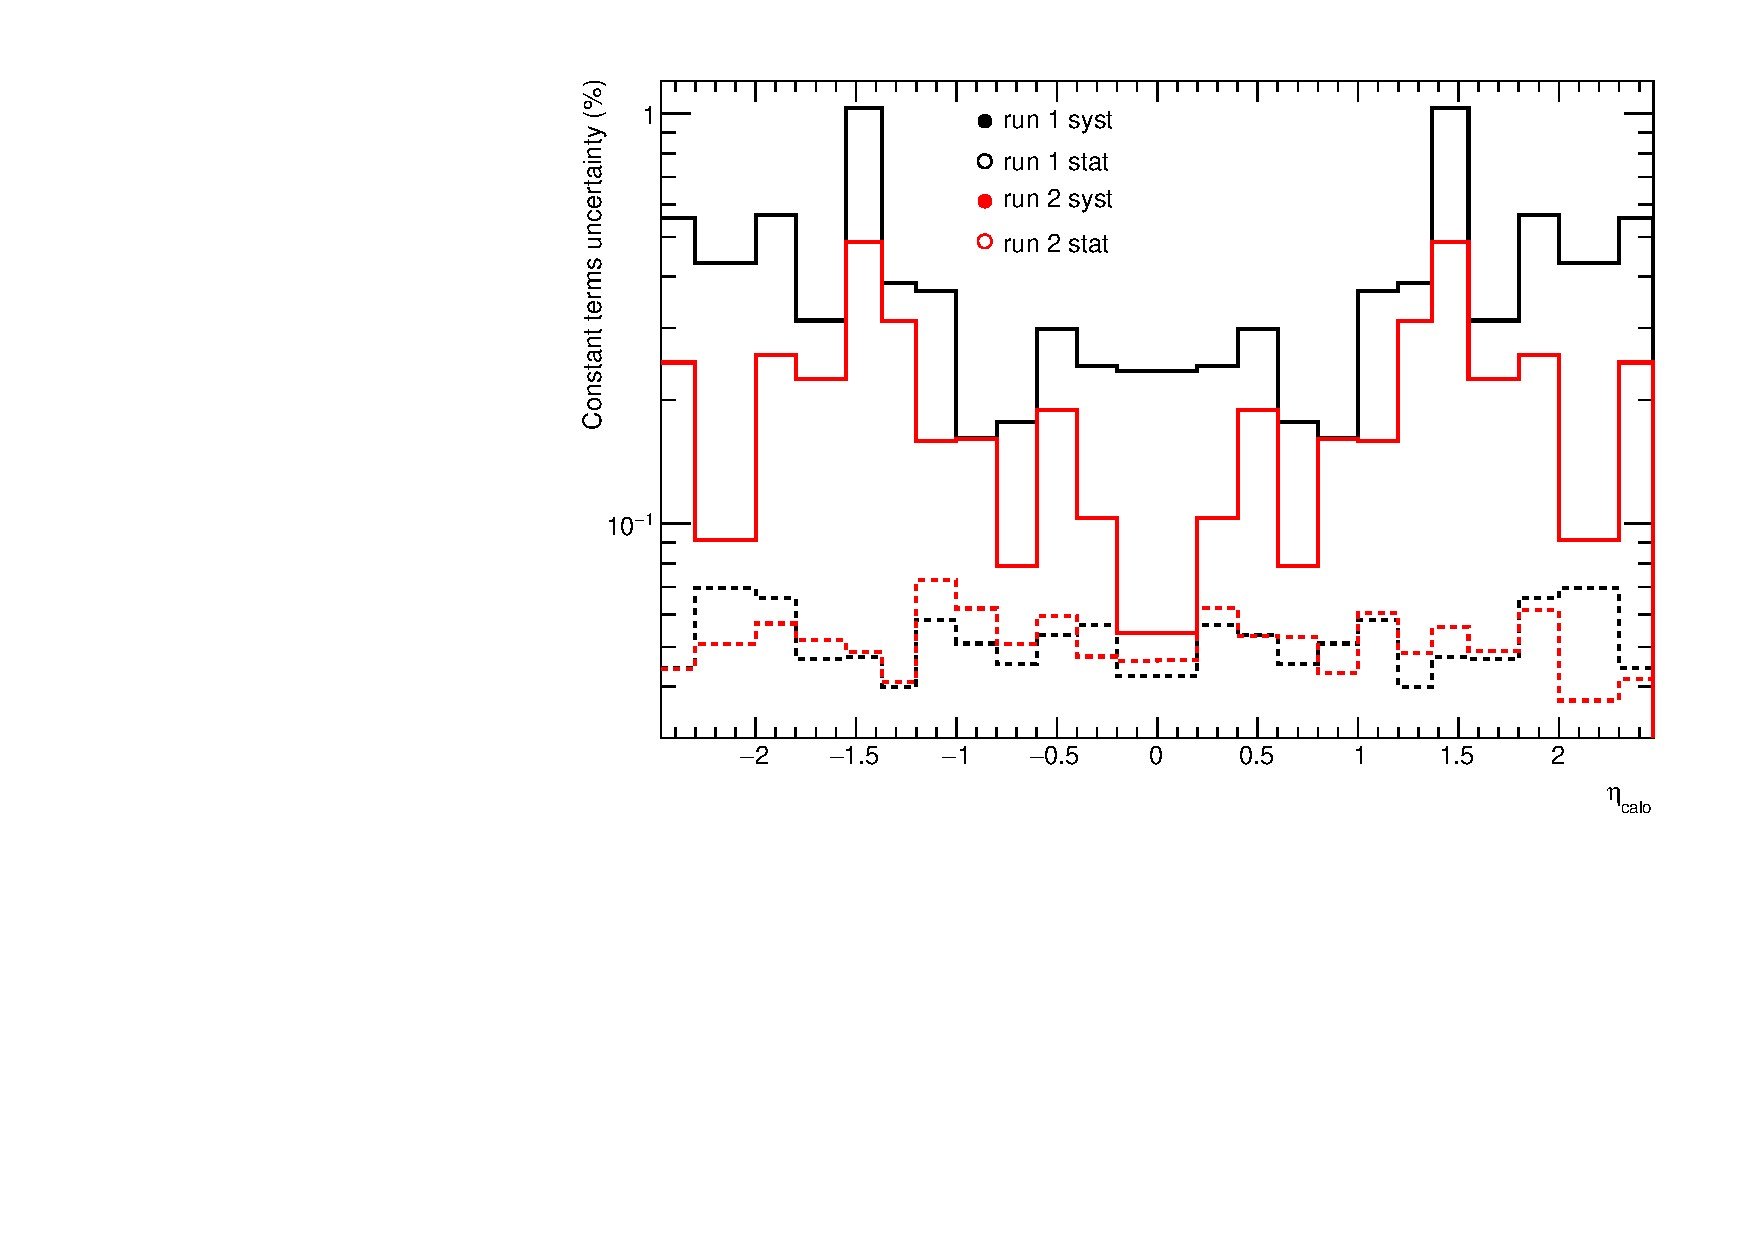
\includegraphics[width=\linewidth]{Figures/CompareSystRun_c.pdf}
  \end{minipage}
  \centering
  \begin{minipage}{0.47\linewidth}
    \includegraphics[width=\linewidth]{CalibSupNote_Distri_m12_corrected.pdf}
  \end{minipage}

\end{frame}

